\documentclass{article}
\usepackage{hyperref}

\usepackage{graphicx}
\usepackage{float}

\usepackage{circuitikz}
\usepackage{pgfplots}
\usepackage{xcolor}
\begin{document}
	
	\begin{titlepage}
		\begin{center}
		\textbf{\huge \color{blue}Electronic Devices And Circuit Theory}
		\line(1,0){300}
		
		\textsc{\huge \color{gray} Diode Applications}\\
		\begin{figure}[h!]
			\centering
			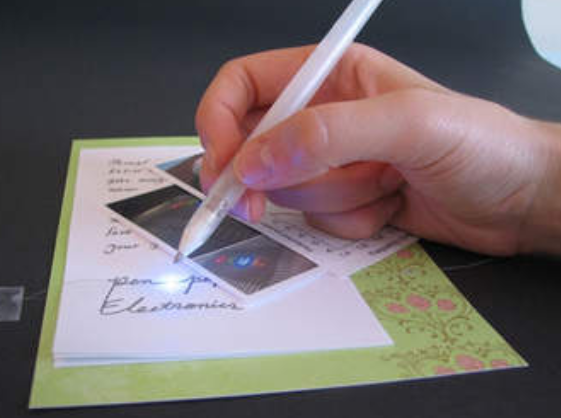
\includegraphics[width=10cm ,height=6cm]{circuit read.png}
		\end{figure}
		
		\end{center}		
		\begin{flushright}
		\textbf{\huge \color{green} Author Information:}\\
		\color{green} \line(1,0){207}\\
			\textsc{\Large Marzia Sultana\\}
			\textsc{Bangabandhu Sheikh Mujibur Rahman Science And Technology University(SHIICT)}\\
			Department Of Computer Science And Engineering\\
			
			ID: 18ICTCSE063\\
			Email: marziasultana57@gmail.com\\
			29 December 2019
		\end{flushright}
		
	\end{titlepage}
	\tableofcontents
	\thispagestyle{empty}

	\section*{summary}
	\addcontentsline{toc}{section}{\numberline{}summary}
	This PDF describes writing report using latex.
	\cleardoublepage
	
	
	\newpage
	\section{Introduction}\label{sec:Intro}
	\line(1,0){300}\\\\
	This chapter will develop a working knowledge of the diode in a variety of the configurations using models appropriate for the area of applications.A diode is a two-terminal electronic component that conducts current primarily in one direction (asymmetric conductance); it has low (ideally zero) resistance in one direction, and high (ideally infinite) resistance in the other. A diode vacuum tube or thermionic diode is a vacuum tube with two electrodes, a heated cathode and a plate, in which electrons can flow in only one direction, from cathode to plate. A semiconductor diode, the most commonly used type today, is a crystalline piece of semiconductor material with a p–n junction connected to two electrical terminals. Semiconductor diodes were the first semiconductor electronic devices. The discovery of asymmetric electrical conduction across the contact between a crystalline mineral and a metal was made by German physicist Ferdinand Braun in 1874. Today, most diodes are made of silicon, but other materials such as gallium arsenide and germanium are also used.\\
	\newpage
	\subsection{History}
	The most common function of a diode is to allow an electric current to pass in one direction (called the diode's forward direction), while blocking it in the opposite direction (the reverse direction). As such, the diode can be viewed as an electronic version of a check valve. This unidirectional behavior is called rectification, and is used to convert alternating current (ac) to direct current (dc). Forms of rectifiers, diodes can be used for such tasks as extracting modulation from radio signals in radio receivers.
	\begin{figure}[H]
		\centering
		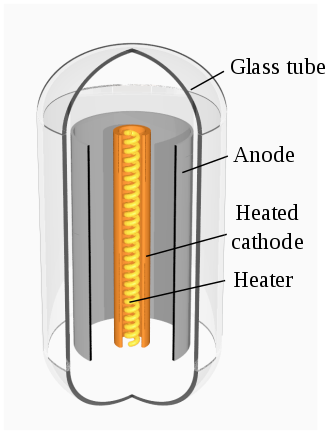
\includegraphics[height=4cm]{330px-Diode-english-text.svg.png}
		\caption{Structure of a vacuum tube diode}
	\end{figure}

However, diodes can have more complicated behavior than this simple on–off action, because of their nonlinear current-voltage characteristics.[7] Semiconductor diodes begin conducting electricity only if a certain threshold voltage or cut-in voltage is present in the forward direction (a state in which the diode is said to be forward-biased). The voltage drop across a forward-biased diode varies only a little with the current, and is a function of temperature; this effect can be used as a temperature sensor or as a voltage reference. Also, diodes' high resistance to current flowing in the reverse direction suddenly drops to a low resistance when the reverse voltage across the diode reaches a value called the breakdown voltage.

A semiconductor diode's current–voltage characteristic can be tailored by selecting the semiconductor materials and the doping impurities introduced into the materials during manufacture.[7] These techniques are used to create special-purpose diodes that perform many different functions.For example, diodes are used to regulate voltage (Zener diodes), to protect circuits from high voltage surges (avalanche diodes), to electronically tune radio and TV receivers (varactor diodes), to generate radio-frequency oscillations (tunnel diodes, Gunn diodes, IMPATT diodes), and to produce light (light-emitting diodes). Tunnel, Gunn and IMPATT diodes exhibit negative resistance, which is useful in microwave and switching circuits.

Diodes, both vacuum and semiconductor, can be used as shot-noise generators.
	\newpage
	\subsection{Semiconductor}
	A semiconductor material has an electrical conductivity value falling between that of a conductor, such as metallic copper, and an insulator, such as glass. Its resistance falls as its temperature rises; metals are the opposite. Its conducting properties may be altered in useful ways by introducing impurities ("doping") into the crystal structure. Where two differently-doped regions exist in the same crystal, a semiconductor junction is created. The behavior of charge carriers which include electrons, ions and electron holes at these junctions is the basis of diodes, transistors and all modern electronics. Some examples of semiconductors are silicon, germanium, gallium arsenide, and elements near the so-called "metalloid staircase" on the periodic table. After silicon, gallium arsenide is the second most common semiconductor[citation needed] and is used in laser diodes, solar cells, microwave-frequency integrated circuits and others. Silicon is a critical element for fabricating most electronic circuits.

Semiconductor devices can display a range of useful properties such as passing current more easily in one direction than the other, showing variable resistance, and sensitivity to light or heat. Because the electrical properties of a semiconductor material can be modified by doping, or by the application of electrical fields or light, devices made from semiconductors can be used for amplification, switching, and energy conversion.

The conductivity of silicon is increased by adding a small amount (of the order of 1 in 108) of pentavalent (antimony, phosphorus, or arsenic) or trivalent (boron, gallium, indium) atoms. This process is known as doping and resulting semiconductors are known as doped or extrinsic semiconductors. Apart from doping, the conductivity of a semiconductor can equally be improved by increasing its temperature. This is contrary to the behaviour of a metal in which conductivity decreases with increase in temperature.

The modern understanding of the properties of a semiconductor relies on quantum physics to explain the movement of charge carriers in a crystal lattice.[1] Doping greatly increases the number of charge carriers within the crystal. When a doped semiconductor contains mostly free holes it is called "p-type", and when it contains mostly free electrons it is known as "n-type". The semiconductor materials used in electronic devices are doped under precise conditions to control the concentration and regions of p- and n-type dopants. A single semiconductor crystal can have many p- and n-type regions; the p–n junctions between these regions are responsible for the useful electronic behavior.
	\newpage
	\subsubsection{P-type and  N-type semiconductor}
	A p-type semiconductor is a type of semiconductor.When the trivalent impurity is added to an intrinsic or pure semiconductor (silicon or germanium), then it is said to be an p-type semiconductor. Trivalent impurities such as Boron (B), Gallium (Ga), Indium(In), Aluminium(Al) etc are called acceptor impurity. Ordinary semiconductors are made of materials that do not conduct (or carry) an electric current very well but are not highly resistant to doing so. They fall half way between conductors and insulators. An electric current occurs when electrons move through a material. In order to move, there must be an electron 'hole' in the material for the electron to move into. A p-type semiconductor has more holes than electrons. This allows the current to flow along the material from hole to hole but only in one direction.

Semiconductors are most often made from silicon. Silicon is an element with four electrons in its outer shell. To make a p-type semiconductor extra materials like boron or aluminium are added to the silicon. These materials have only three electrons in their outer shell. When the extra material replaces some of the silicon it leaves a 'hole' where the fourth electron would have been if the semiconductor was pure silicon.
An N-type semiconductor is a type of material used in electronics.

It is made by adding an impurity to a pure semiconductor such as silicon or germanium. The impurities used may be phosphorus, arsenic, antimony, bismuth or some other chemical element. They are called donor impurities. The impurity is called a donor because it gives a free electron to a semiconductor. The purpose of doing this is to make more charge carriers, or electron wires available in the material for conduction. The final material is a lot more conductive than the original silicon or germanium.
\newpage
	\subsection{P-N Junction Diode}
	A p-n junction diode is two-terminal or two-electrode semiconductor device, which allows the electric current in only one direction while blocks the electric current in opposite or reverse direction. If the diode is forward biased, it allows the electric current flow. On the other hand, if the diode is reverse biased, it blocks the electric current flow. P-N junction semiconductor diode is also called as p-n junction semiconductor device.

In n-type semiconductors, free electrons are the majority charge carriers whereas in p-type semiconductors, holes are the majority charge carriers. When the n-type semiconductor is joined with the p-type semiconductor, a p-n junction is formed. The p-n junction, which is formed when the p-type and n-type semiconductors are joined, is called as p-n junction diode.

The p-n junction diode is made from the semiconductor materials such as silicon, germanium, and gallium arsenide. For designing the diodes, silicon is more preferred over germanium. The p-n junction diodes made from silicon semiconductors works at higher temperature when compared with the p-n junction diodes made from germanium semiconductors.

The basic symbol of p-n junction diode under forward and reverse bias is shown in the below figure
	\begin{figure}[h!]
	\centering
		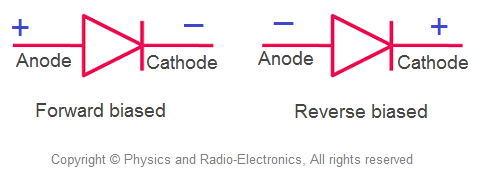
\includegraphics[height=4cm]{symbolofdiode.png}
	\caption{p-n junction diode}
	\end{figure}

In the above figure, arrowhead of a diode indicates the conventional direction of electric current when the diode is forward biased (from positive terminal to the negative terminal). The holes which moves from positive terminal (anode) to the negative terminal (cathode) is the conventional direction of current.

The free electrons moving from negative terminal (cathode) to the positive terminal (anode) actually carry the electric current. However, due to the convention we have to assume that the current direction is from positive terminal to the negative terminal.
\subparagraph{\large Terminals of diode under forward bias:}
In forward biased p-n junction diode (p-type connected to positive terminal and n-type connected to negative terminal), anode terminal is a positive terminal whereas cathode terminal is negative terminal.

Anode terminal is a positively charged electrode or conductor, which supplies holes to the p-n junction. In other words, anode or anode terminal or positive terminal is the source of positive charge carriers (holes), the positive charge carriers (holes) begins their journey at anode terminal and travel through the diode and ends at cathode terminal.
\begin{figure}[H]
	\centering
	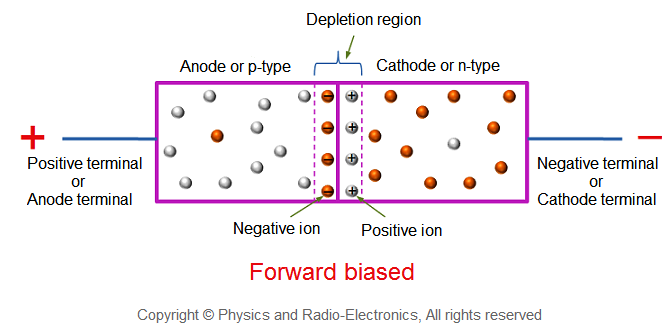
\includegraphics[height=5cm]{terminalsunderforward.png}
	\caption{Forward biase}
\end{figure}

 Cathode is the negatively charged electrode or conductor, which supplies free electrons to the p-n junction.             
Cathode is the negatively charged electrode or conductor, which supplies free electrons to the p-n junction. In other words, cathode terminal or negative terminal is the source of free electrons, the negative charge carriers (free electrons) begins their journey at cathode terminal and travel through the diode and ends at anode terminal.

The free electrons are attracted towards the anode terminal or positive terminal whereas the holes are attracted towards the cathode terminal or negative terminal.

\subparagraph{\large Terminals of diode under reverse bias:} 
If the diode is reverse biased (p-type connected to negative terminal and n-type connected to positive terminal), the anode terminal becomes a negative terminal whereas the cathode terminal becomes a positive terminal.

Anode terminal or negative terminal supplies free electrons to the p-n junction. In other words, anode terminal is the source of free electrons, the free electrons begins their journey at negative or anode terminal and fills the large number of holes in the p-type semiconductor. The holes in the p-type semiconductor get attracted towards the negative terminal. The free electrons from the negative terminal cannot move towards the positive terminal because the wide depletion region at the p-n junction resists or opposes the flow of free electrons.
\begin{figure}[H]
	\centering
	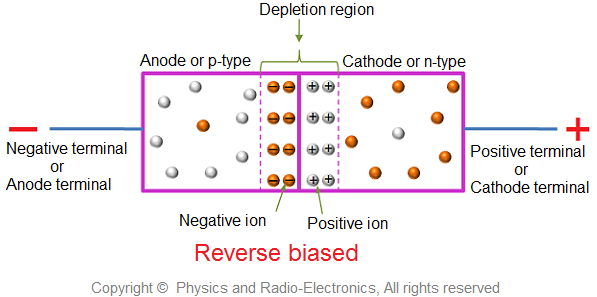
\includegraphics[height=5cm]{terminalsreversebias.png}
	\caption{Reverse biase}
\end{figure}

Cathode terminal or positive terminal supplies holes to the p-n junction. In other words, cathode terminal is the source of holes
Cathode terminal or positive terminal supplies holes to the p-n junction. In other words, cathode terminal is the source of holes, the holes begins their journey at positive or cathode terminal and occupies the electrons position in the n-type semiconductor. The free electrons in the n-type semiconductor gets attracted towards the positive terminal. The holes from the positive terminal cannot move towards the negative terminal because the wide depletion region at the p-n junction opposes the flow of holes.
	\subsection{Rectifier Concept}
	{\large What is Rectification?}
	
	
Now we come to the most popular application of the diode: rectification. Simply defined, rectification is the conversion of alternating current (AC) to direct current (DC). This involves a device that only allows one-way flow of electric charge. As we have seen, this is exactly what a semiconductor diode does. The simplest kind of rectifier circuit is the half-wave rectifier. It only allows one half of an AC waveform to pass through to the load. (Figure below)
	\begin{figure}[H]
		\centering
		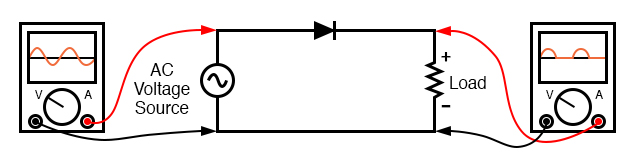
\includegraphics[height=3cm]{half-wave-rectifier-circuit.jpg}
		\caption{Half wave rectifier circuit}
	\end{figure}
	\subsection{Half Wave Rectification}
	For most power applications, half-wave rectification is insufficient for the task. The harmonic content of the rectifier’s output waveform is very large and consequently difficult to filter. Furthermore, the AC power source only supplies power to the load one half every full cycle, meaning that half of its capacity is unused. Half-wave rectification is, however, a very simple way to reduce power to a resistive load. Some two-position lamp dimmer switches apply full AC power to the lamp filament for “full” brightness and then half-wave rectify it for a lesser light output. (figure below)
	\begin{figure}[h]
	\begin{center}
		\begin{circuitikz}
			\draw(0,0)
			to[V,v=$U_q$](0,2)
			to[short](2,2)
			to[R=$R_1$](2,0)
			to[short](0,0);
		\end{circuitikz}
		\caption{half wave rectifier}
	\end{center}
	\end{figure}
	
	
	Half-wave rectifier application: Two level lamp dimmer.

In the “Dim” switch position, the incandescent lamp receives approximately one-half the power it would normally receive operating on full-wave AC. Because the half-wave rectified power pulses far more rapidly than the filament has time to heat up and cool down, the lamp does not blink. Instead, its filament merely operates at a lesser temperature than normal, providing less light output.\\
 \begin{tabular}{|c|c|c|}
    \hline
    column1 &column2 &column3\\\hline
    zener diode &tanel diode &photo diode\\\hline
    \end{tabular}

This principle of “pulsing” power rapidly to a slow-responding load device to control the electrical power sent to it is common in the world of industrial electronics. Since the controlling device (the diode, in this case) is either fully conducting or fully nonconducting at any given time, it dissipates little heat energy while controlling load power, making this method of power control very energy-efficient. This circuit is perhaps the crudest possible method of pulsing power to a load, but it suffices as a proof-of-concept application.


	
	\subsection{Full Wave Rectification}
	
	If we need to rectify AC power to obtain the full use of both half-cycles of the sine wave, a different rectifier circuit configuration must be used. Such a circuit is called a full-wave rectifier. One kind of full-wave rectifier, called the center-tap design, uses a transformer with a center-tapped secondary winding and two diodes, as in the figure below.
	\begin{figure}[H]
		\centering
		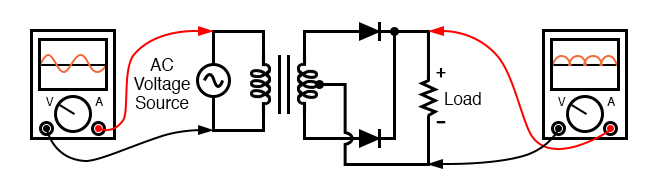
\includegraphics[height=3cm]{full-waive-rectifier-center-tapped-design.jpg}
		\caption{Full wave rectifier,center trap design}
	\end{figure}
	{\large Positive Half-Cycle:}\\
This circuit’s operation is easily understood one half-cycle at a time. Consider the first half-cycle, when the source voltage polarity is positive (+) on top and negative (-) on bottom. At this time, only the top diode is conducting; the bottom diode is blocking current, and the load “sees” the first half of the sine wave, positive on top and negative on bottom. Only the top half of the transformer’s secondary winding carries current during this half-cycle as in the figure below.
	\begin{figure}[H]
		\centering
		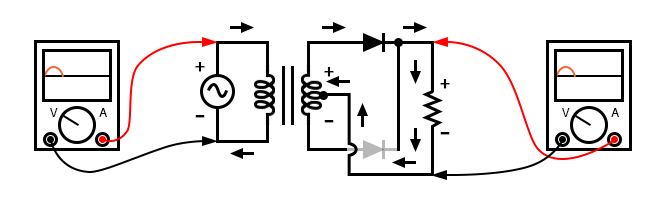
\includegraphics[height=3cm]{full-wave-center-tap-rectifier-positive-half-cycle.jpg}
		\caption{Positive half cycle}
	\end{figure}
Full-wave center-tap rectifier: Top half of secondary winding conducts during positive half-cycle of input, delivering positive half-cycle to load.\\


	{\large Negative Half-Cycle}\\
During the next half-cycle, the AC polarity reverses. Now, the other diode and the other half of the transformer’s secondary winding carry current while the portions of the circuit formerly carrying current during the last half-cycle sit idle. The load still “sees” half of a sine wave, of the same polarity as before: positive on top and negative on bottom. (Figure below)
	\begin{figure}[H]
		\centering
		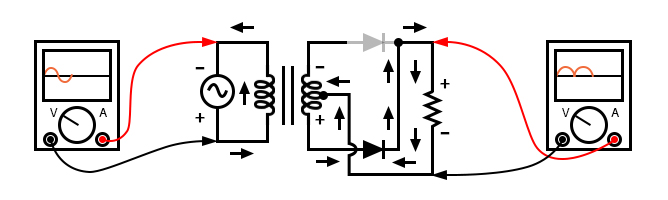
\includegraphics[height=3cm]{full-wave-center-tap-rectifier-negative-half-cycle.jpg}
		\caption{Negative half cycle}
	\end{figure}

Full-wave center-tap rectifier: During negative input half-cycle, bottom half of secondary winding conducts, delivering a positive half-cycle to the load.
	\subsection{Clipers}
	In electronics, a clipper is a circuit designed to prevent a signal from exceeding a predetermined reference voltage level. A clipper does not distort the remaining part of the applied waveform. Clipping circuits are used to select, for purposes of transmission, that part of a signal waveform which lies above or below the predetermined reference voltage level.

Clipping may be achieved either at one level or two levels. A clipper circuit can remove certain portions of an arbitrary waveform near the positive or negative peaks or both. Clipping changes the shape of the waveform and alters its spectral components.

A clipping circuit consists of linear elements like resistors and non-linear elements like diodes or transistors, but it does not contain energy-storage elements like capacitors.

Clipping circuits are also called slicers or amplitude selectors.


\paragraph{\large Diode clipper\\}
Positive peak clipper circuit
A simple diode clipper can be made with a diode and a resistor. This will remove either the positive, or the negative half of the waveform depending on the direction the diode is connected. The simple circuit clips at zero voltage (or to be more precise, at the small forward voltage of the forward biased diode) but the clipping voltage can be set to any desired value with the addition of a reference voltage. The diagram illustrates a positive reference voltage but the reference can be positive or negative for both positive and negative clipping giving four possible configurations in all.

The simplest circuit for the voltage reference is a resistor potential divider connected between the voltage rails. This can be improved by replacing the lower resistor with a zener diode with a breakdown voltage equal to the required reference voltage. The zener acts as a voltage regulator stabilising the reference voltage against supply and load variations.
\begin{figure}[H]
		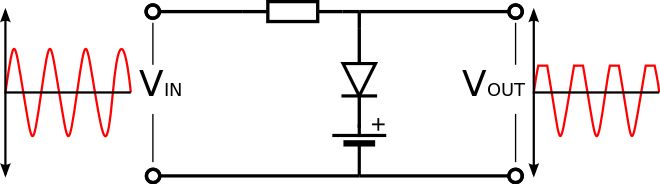
\includegraphics[height=3cm]{660px-Diode_Voltage_Clipper.svg.png}
		\caption{Diode clipper}
	\end{figure}

\paragraph{\large Zener diode\\} 
Two shunt zener-diode clipper circuits
Two shunt diode clipper circuit
In the example circuit on the right, two zener diodes are used to clip the voltage VIN. The voltage in either direction is limited to the reverse breakdown voltage plus the forward voltage drop across one zener diode.
\begin{figure}[H]
		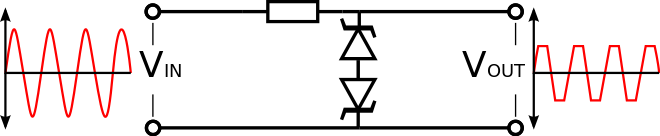
\includegraphics[height=3cm]{660px-Zener_Diode.svg.png}
		\caption{Zener clipper}
	\end{figure}

\paragraph{\large Op-amp precision clipper\\} 
For very small values of clipping voltage on low-level signals the I-V curve of the diode can result in clipping onset that is not very sharp. Precision clippers can be made by placing the clipping device in the feedback circuit of an operational amplifier in a manner similar to precision rectifiers.
\paragraph{\huge Classification\\}
Clippers may be classified into two types based on the positioning of the diode. 

Series clippers, where the diode is in series with the load resistance, and
Shunt clippers, where the diode is shunted across the load resistance.
The diode capacitance affects the operation of the clipper at high frequency and influences the choice between the above two types. High frequency signals are attenuated in the shunt clipper as the diode capacitance provides an alternative path to output current. In the series clipper, clipping effectiveness is reduced for the same reason as the high frequency current passes through without being sufficiently blocked.

Clippers may be classified based on the orientation of the diode. The orientation decides which half cycle is affected by the clipping action.

The clipping action can be made to happen at an arbitrary level by using a biasing element (potential source) in series with the diode. In the following diagrams the green plot is the input voltage, the orange plot is the output voltage, and the blue plot is the clipping level voltage.

\large Positively biased diode clipper:\\

\begin{figure}[H]
\begin{tikzpicture}[x=10cm]
    \begin{axis}[    	
        xmin=-0.5,xmax=10,
        ymin=-10,ymax=10,
        axis x line=middle,
        axis y line=middle,
        axis line style=<->,
        xlabel={$U_i$},
        ylabel={$U_{im}$},
        ]
        \addplot[ no marks,blue,<->] expression[domain=-2*pi:pi,samples=100]{sin(deg(3*x))+1/4} 
        node[pos=0.90,anchor=south west]{$U_i(x)=U_{im}sin(0.5x)$}; 
   	\end{axis}
\end{tikzpicture}
\caption{Input graph}
\end{figure}

\begin{figure}[H]
\centering
	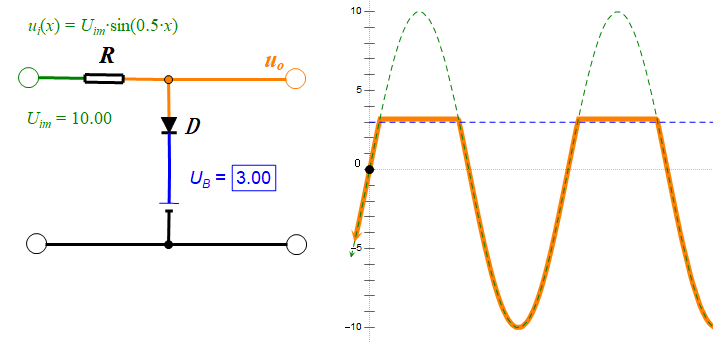
\includegraphics[height=3cm]{wave.png}
	\caption{Output graph}
\end{figure}



	
	\subsection{\large Clampers}
	\large{Clamper definition\\}
A clamper is an electronic circuit that changes the DC level of a signal to the desired level without changing the shape of the applied signal. In other words, the clamper circuit moves the whole signal up or down to set either the positive peak or negative peak of the signal at the desired level.

The dc component is simply added to the input signal or subtracted from the input signal. A clamper circuit adds the positive dc component to the input signal to push it to the positive side. Similarly, a clamper circuit adds the negative dc component to the input signal to push it to the negative side.
\begin{figure}[H]
	\centering
	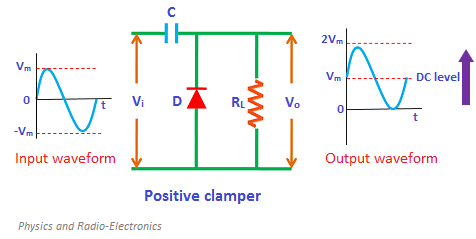
\includegraphics[height=3cm]{positiveclamper.png}
	\caption{positive clamper}
\end{figure}

If the circuit pushes the signal upwards then the circuit is said to be a positive clamper.
If the circuit pushes the signal upwards then the circuit is said to be a positive clamper. When the signal is pushed upwards, the negative peak of the signal meets the zero level.
\begin{figure}[H]
	\centering
	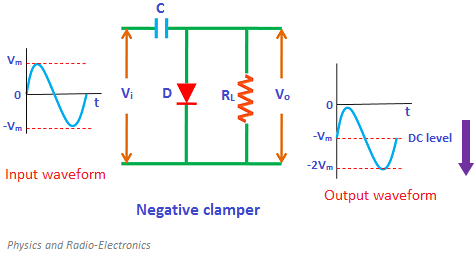
\includegraphics[height=3cm]{negativeclamper.png}
	\caption{negative clamper}
\end{figure}

On the other hand, if the circuit pushes the signal downwards then the circuit is said to be a negative clamper.
On the other hand, if the circuit pushes the signal downwards then the circuit is said to be a negative clamper. When the signal is pushed downwards, the positive peak of the signal meets the zero level.

The construction of the clamper circuit is almost similar to the clipper circuit. The only difference is the clamper circuit contains an extra element called capacitor. A capacitor is used to provide a dc offset (dc level) from the stored charge.

A typical clamper is made up of a capacitor, diode, and resistor. Some clampers contain an extra element called DC battery. The resistors and capacitors are used in the clamper circuit to maintain an altered DC level at the clamper output. The clamper is also referred to as a DC restorer, clamped capacitors, or AC signal level shifter.

Types of clampers
Clamper circuits are of three types:

Positive clampers
Negative clampers
Biased clampers
Positive clamper
The positive clamper is made up of a voltage source Vi, capacitor C, diode D, and load resistor RL. In the below circuit diagram, the diode is connected in parallel with the output load. So the positive clamper passes the input signal to the output load when the diode is reverse biased and blocks the input signal when the diode is forward biased.

During the negative half cycle of the input AC signal, the diode is forward biased and hence no signal appears at the output. 
\begin{figure}[H]
	\centering
	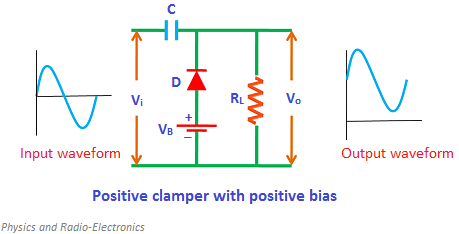
\includegraphics[height=3cm]{positiveclamperwithpositivebias.png}
	\caption{positive clamper with positive bias}
\end{figure}
During negative half cycle:

During the negative half cycle of the input AC signal, the diode is forward biased and hence no signal appears at the output. In forward biased condition, the diode allows electric current through it. This current will flows to the capacitor and charges it to the peak value of input voltage Vm. The capacitor charged in inverse polarity (positive) with the input voltage. As input current or voltage decreases after attaining its maximum value -Vm, the capacitor holds the charge until the diode remains forward biased.

During positive half cycle:

During the positive half cycle of the input AC signal, the diode is reverse biased and hence the signal appears at the output. In reverse biased condition, the diode does not allow electric current through it. So the input current directly flows towards the output.


When the positive half cycle begins, the diode is in the non-conducting state and the charge stored in the capacitor is discharged (released). Therefore, the voltage appeared at the output is equal to the sum of the voltage stored in the capacitor (Vm) and the input voltage (Vm) { I.e. Vo = Vm+ Vm = 2Vm} which have the same polarity with each other. As a result, the signal shifted upwards.

The peak to peak amplitude of the input signal is 2Vm, similarly the peak to peak amplitude of the output signal is also 2Vm. Therefore, the total swing of the output is same as the total swing of the input.

The basic difference between the clipper and clamper is that the clipper removes the unwanted portion of the input signal whereas the clamper moves the input signal upwards or downwards.


Negative clamper
During positive half cycle:

During the positive half cycle of the input AC signal, the diode is forward biased and hence no signal appears at the output. In forward biased condition, the diode allows electric current through it. This current will flows to the capacitor and charges it to the peak value of input voltage in inverse polarity -Vm. As input current or voltage decreases after attaining its maximum value Vm, the capacitor holds the charge until the diode remains forward biased.

During the positive half cycle of the input AC signal, the diode is forward biased and hence no signal appears at the output. 
During negative half cycle:

During the negative half cycle of the input AC signal, the diode is reverse biased and hence the signal appears at the output. In reverse biased condition, the diode does not allow electric current through it. So the input current directly flows towards the output.

When the negative half cycle begins, the diode is in the non-conducting state and the charge stored in the capacitor is discharged (released). Therefore, the voltage appeared at the output is equal to the sum of the voltage stored in the capacitor (-Vm) and the input voltage (-Vm) {I.e. Vo = -Vm- Vm = -2Vm} which have the same polarity with each other. As a result, the signal shifted downwards.

Biased clampers
Sometimes an additional shift of DC level is needed. In such cases, biased clampers are used. The working principle of the biased clampers is almost similar to the unbiased clampers. The only difference is an extra element called DC battery is introduced in biased clampers.

Positive clamper with positive bias
If positive biasing is applied to the clamper then it is said to be a positive clamper with positive bias. The positive clamper with positive bias is made up of an AC voltage source, capacitor, diode, resistor, and dc battery.

During positive half cycle:

During the positive half cycle, the battery voltage forward biases the diode when the input supply voltage is less than the battery voltage. This current or voltage will flows to the capacitor and charges it.

When the input supply voltage becomes greater than the battery voltage then the diode stops allowing electric current through it because the diode becomes reverse biased.

If positive biasing is applied to the clamper then it is said to be a positive clamper with positive bias.
During negative half cycle:

During the negative half cycle, the diode is forward biased by both input supply voltage and battery voltage. So the diode allows electric current. This current will flows to the capacitor and charges it.

Positive clamper with negative bias
During negative half cycle:

During the negative half cycle, the battery voltage reverse biases the diode when the input supply voltage is less than the battery voltage. As a result, the signal appears at the output.

When the input supply voltage becomes greater than the battery voltage, the diode is forward biased by the input supply voltage and hence allows electric current through it. This current will flows to the capacitor and charges it.

During the negative half cycle, the battery voltage reverse biases the diode when the input supply voltage is less than the battery voltage. As a result, signal appears at the output.
During positive half cycle:

During the positive half cycle, the diode is reverse biased by both input supply voltage and the battery voltage. As a result, the signal appears at the output. The signal appeared at the output is equal to the sum of the input voltage and capacitor voltage.

Negative clamper with positive bias
During positive half cycle:

During the positive half cycle, the battery voltage reverse biases the diode when the input supply voltage is less than the battery voltage. When the input supply voltage becomes greater than the battery voltage, the diode is forward biased by the input supply voltage and hence allows electric current through it. This current will flows to the capacitor and charges it.

During the positive half cycle, the battery voltage reverse biases the diode when the input supply voltage is less than the battery voltage. 
During negative half cycle:

During the negative half cycle, the diode is reverse biased by both input supply voltage and battery voltage. As a result, the signal appears at the output.
\begin{figure}[H]
	\centering
	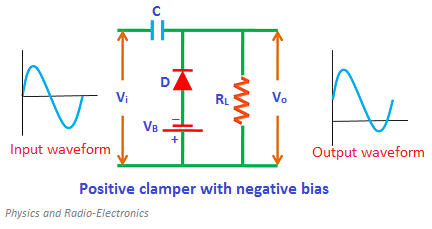
\includegraphics[height=3cm]{positiveclamperwithnegativebias.png}
	\caption{positive clamper with negative bias}
\end{figure}

Negative clamper with negative bias
During positive half cycle:

During the positive half cycle, the diode is forward biased by both input supply voltage and battery voltage. As a result, current flows through the capacitor and charges it.

During the positive half cycle, the diode is forward biased by both input supply voltage and battery voltage. As a result, current flows through the capacitor and charges it.
During negative half cycle:

During the negative half cycle, the battery voltage forward biases the diode when the input supply voltage is less than the battery voltage. When the input supply voltage becomes greater than the battery voltage, the diode is reverse biased by the input supply voltage and hence signal appears at the output.
\clearpage
	\addcontentsline{toc}{section}{\refname}

\newpage
\textbf{\huge Reference}\\
this reference is
\url{<https://www.researchgate.net/post/In_Latex_how_do_I_create_citations_to_references_with_a_hyperlink>}	
,\\ 
\url{<https://www.latex-tutorial.com/tutorials/circuitikz/>},\\\url{<https://www.daenotes.com/electronics/digital-electronics/clipper-circuits>},\\ \url{<https://en.wikipedia.org/wiki/Clipper_(electronics)>},\\ \url{<https://en.wikipedia.org/wiki/PE28093n_junction>},\\ \url{<https://www.electronics-tutorials.ws/diode/diode_3.html>}

	
\end{document}
